\chapter{Multi-period optimal power flow (TCOPFLOW)}\label{chap:tcopflow}

TCOPFLOW solves a full AC multi-period optimal power flow problem with the objective of minimizing the total cost over the given time horizon while adhering to constraints for each period and between consecutive time-periods (ramping constraints). 

\section{Formulation}
The multi-period optimal power flow problem is a series of optimal power flow problems coupled via temporal constraints. The generator real power deviation ($p_{jt}^{\text{g}} - p_{jt-\Delta{t}}^{\text{g}}$) constrained within the ramp limits form the temporal constraints. An illustration of the temporal constraints is shown in Fig. \ref{fig:tcopflow} with four time steps. Each time-step $t$ is coupled with its preceding time $t-\Delta{t}$, where $\Delta{t}$ is the time-step where the objective is to find a least cost dispatch for the given time horizon.

\definecolor{lavander}{cmyk}{0,0.48,0,0}
\definecolor{violet}{cmyk}{0.79,0.88,0,0}
\definecolor{burntorange}{cmyk}{0,0.52,1,0}

\def\lav{lavander!90}
\def\oran{orange!30}

\tikzstyle{time}=[draw,circle,violet,bottom color=\lav,
                  top color= white, text=violet,minimum width=20pt]
\tikzstyle{base}=[draw,circle,burntorange, left color=\oran,
                       text=violet,minimum width=20pt]

\begin{figure}[h!]
\centering
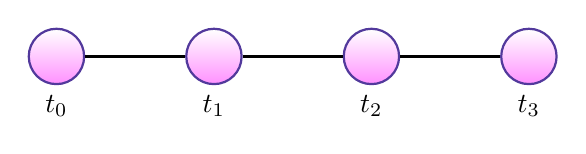
\begin{tikzpicture}[auto, thick]
  \node[time,label=below:$t_0$] (t0) at (0,0) {};
  \node[time,label=below:$t_1$] (t1) at (2,0) {};
  \node[time,label=below:$t_2$] (t2) at (4,0) {};
  \node[time,label=below:$t_3$] (t3) at (6,0) {};
  
  \path (t0) edge (t1);
  \path (t1) edge (t2);
  \path (t2) edge (t3);


\end{tikzpicture}
\caption{Multi-period optimal power flow example with four time-steps. The lines connecting the different time-periods denote the coupling between them.}
\label{fig:tcopflow}
\end{figure}


In general form, the equations for multi-period optimal power flow are given by
(\ref{eq:tcopflow_start}) -- (\ref{eq:tcopflow_end}). TCOPFLOW solves to
minimize the total generation cost $\sum_{t=0}^{N_t-1}f(x_t)$ over the time
horizon, where $N_t$ is the number of time-steps. At each time-step, the
equality constraints ($g(x_t)$), inequality $h(x_t)$, and the lower/upper limit
($x^-$,$x^+$) constraints need to be satisfied. Equation (\ref{eq:tcopflow_end})
represents the coupling between the consecutive time-steps. It is the most
common form of coupling that limits the deviation of the real power generation
at time $t$ from its preceding time-step $t-\Delta{t}$ to within its ramping
capability $\Delta x_t$.


\begin{align}
\centering
\text{min}&~\sum_{t=0}^{N_t-1} f(x_t) &  \label{eq:tcopflow_start}\\
&\text{s.t.}& \nonumber \\
&~g(x_t) = 0,                                        &t \in \left[0,N_t-1\right]& \\
&~h(x_t) \le 0,                                      &t \in \left[0,N_t-1\right]& \\
x^- & \le x_t \le x^+,                               &t\in \left[0,N_t-1\right]& \\
-\Delta x_t & \le x_t - x_{t-\Delta{t}} \le \Delta x_t,&t \in \left[1,N_t-1\right]&
\label{eq:tcopflow_end}
\end{align}

\section{Solvers}\label{sec:tcopflow_solvers}%
Currently, \exago only supports solving \tcopflow using \ipopt~ on on a single rank. %Option:\\ %\opflowoption{-tcopflow_solver IPOPT}

\section{Input and Output}
\begin{itemize}
    \item \textbf{Network file:} The network file describing the network details. Only \matpower format files are currently supported.
    \item \textbf{Load data:} One file for load real power and one for reactive power. The files need to be in CSV format. An example of the format for the 9-bus case is \href{https://gitlab.pnnl.gov/exasgd/frameworks/exago/-/tree/master/datafiles/case9}{here}.
    \item \textbf{Wind generation:} The wind generation time-series described in CSV format. See an example of the format \href{https://gitlab.pnnl.gov/exasgd/frameworks/exago/-/tree/master/datafiles/case9}{here}.
\end{itemize}
If the load data and/or wind generation profiles are not set then a flat profile is assumed, i.e., the load and wind generation for all hours is constant.

The \tcopflow output is saved to a directory named \texttt{tcopflowout}. This directory contains $N_t$ files, one for each time-step, in \matpower data file format.

\section{Usage}
\begin{lstlisting}
./bin/tcopflow -netfile $EXAGO_DIR/datafiles/case9/case9mod.m -tcopflow_ploadprofile $EXAGO_DIR/datafiles/case9/load_P.csv -tcopflow_qloadprofile $EXAGO_DIR/datafiles/case9/load_Q.csv -print_output -tcopflow_dT 5 -tcopflow_duration 0.5
[ExaGO] TCOPFLOW: Application created
[ExaGO] TCOPFLOW: Duration = 0.500000 hours, timestep = 5.000000 minutes, number of time-steps = 7
[ExaGO] TCOPFLOW: Using IPOPT solver
[ExaGO] TCOPFLOW: Setup completed

******************************************************************************
This program contains Ipopt, a library for large-scale nonlinear optimization.
 Ipopt is released as open source code under the Eclipse Public License (EPL).
         For more information visit http://projects.coin-or.org/Ipopt
******************************************************************************

This is Ipopt version 3.12.10, running with linear solver ma27.

Number of nonzeros in equality constraint Jacobian...:      798
Number of nonzeros in inequality constraint Jacobian.:      540
Number of nonzeros in Lagrangian Hessian.............:      672

Total number of variables............................:      168
                     variables with only lower bounds:        0
                variables with lower and upper bounds:      112
                     variables with only upper bounds:        0
Total number of equality constraints.................:      126
Total number of inequality constraints...............:      144
        inequality constraints with only lower bounds:        0
   inequality constraints with lower and upper bounds:      144
        inequality constraints with only upper bounds:        0

iter    objective    inf_pr   inf_du lg(mu)  ||d||  lg(rg) alpha_du alpha_pr  ls
   0  7.2226875e+04 1.80e+00 1.00e+02  -1.0 0.00e+00    -  0.00e+00 0.00e+00   0
   1  5.1460539e+04 1.04e+00 1.60e+02  -1.0 1.08e+00    -  6.27e-01 4.21e-01f  1
   2  4.8692257e+04 9.13e-01 1.60e+03  -1.0 1.42e+00   2.0 2.84e-03 1.29e-01f  1
   3  4.1695179e+04 5.82e-01 8.63e+02  -1.0 1.09e+00    -  3.86e-03 3.78e-01f  1
   4  3.8223523e+04 4.01e-01 5.86e+02  -1.7 7.91e-01    -  2.00e-01 3.10e-01f  1
   5  3.1081047e+04 9.06e-02 1.98e+03  -1.7 5.58e-01    -  4.80e-01 1.00e+00f  1
   6  3.0468392e+04 1.83e-01 1.34e+02  -1.7 5.84e-01    -  2.75e-01 1.00e+00f  1
   7  3.0405940e+04 9.33e-02 4.47e+00  -1.7 3.04e-01    -  4.96e-01 1.00e+00f  1
   8  3.0382232e+04 3.12e-02 7.07e-01  -2.5 1.76e-01    -  7.33e-01 1.00e+00h  1
   9  3.0369124e+04 2.45e-03 4.69e-02  -2.5 4.46e-02    -  1.00e+00 1.00e+00h  1
iter    objective    inf_pr   inf_du lg(mu)  ||d||  lg(rg) alpha_du alpha_pr  ls
  10  3.0364520e+04 9.81e-04 7.50e-02  -3.8 2.34e-02    -  9.84e-01 6.75e-01h  1
  11  3.0364301e+04 1.91e-04 1.14e-02  -3.8 1.67e-02    -  8.91e-01 9.19e-01h  1
  12  3.0364426e+04 4.32e-05 9.33e-05  -3.8 6.82e-03    -  1.00e+00 1.00e+00f  1
  13  3.0364326e+04 1.45e-05 4.77e-03  -5.7 3.90e-03    -  1.00e+00 9.44e-01h  1
  14  3.0364329e+04 1.12e-06 2.32e-06  -5.7 1.10e-03    -  1.00e+00 1.00e+00h  1
  15  3.0364328e+04 7.91e-09 3.33e-08  -7.0 9.28e-05    -  1.00e+00 1.00e+00h  1

Number of Iterations....: 15

                                   (scaled)                 (unscaled)
Objective...............:   6.8081453631121144e+02    3.0364328319480031e+04
Dual infeasibility......:   3.3330834427063850e-08    1.4865552154470478e-06
Constraint violation....:   1.5610245006347778e-09    1.5610245006347778e-09
Complementarity.........:   1.0802025033126202e-07    4.8177031647742860e-06
Overall NLP error.......:   1.0802025033126202e-07    4.8177031647742860e-06


Number of objective function evaluations             = 16
Number of objective gradient evaluations             = 16
Number of equality constraint evaluations            = 16
Number of inequality constraint evaluations          = 16
Number of equality constraint Jacobian evaluations   = 16
Number of inequality constraint Jacobian evaluations = 16
Number of Lagrangian Hessian evaluations             = 15
Total CPU secs in IPOPT (w/o function evaluations)   =      0.036
Total CPU secs in NLP function evaluations           =      0.014

EXIT: Optimal Solution Found.
=============================================================
Multi-Period Optimal Power Flow
=============================================================
OPFLOW Model                        POWER_BALANCE_POLAR
Solver                              IPOPT
Duration (minutes)                  30.00
Time-step (minutes)                 5.00 
Number of steps                     7
Active power demand profile         /people/abhy245/projects/exaSGD/exago/datafiles/case9/load_P.csv
Rective power demand profile        /people/abhy245/projects/exaSGD/exago/datafiles/case9/load_Q.csv
Wind generation profile             NOT SET
Load loss allowed                   NO
Power imbalance allowed             NO
Ignore line flow constraints        NO

Number of variables                 168
Number of equality constraints      126
Number of inequality constraints    126
Number of coupling constraints      18

Convergence status                  CONVERGED
Objective value                     30364.33

----------------------------------------------------------------------
Bus        Pd      Qd      Vm      Va      mult_Pmis      mult_Qmis      Pslack         Qslack        
----------------------------------------------------------------------
1         0.00    0.00   1.089   0.000      2102.34        -0.00         0.00         0.00
2         0.00    0.00   1.092   3.904      2059.04        -0.00         0.00         0.00
3         0.00    0.00   1.087   2.077      2065.00        -0.00         0.00         0.00
4         0.00    0.00   1.095  -2.016      2102.60        -0.04         0.00         0.00
5        75.00   30.00   1.088  -3.150      2112.60         1.16         0.00         0.00
6        90.00   30.00   1.085  -3.962      2129.51         1.68         0.00         0.00
7         0.00    0.00   1.100   0.501      2059.43        -0.06         0.00         0.00
8       100.00   35.00   1.089  -1.757      2079.19         2.98         0.00         0.00
9         0.00    0.00   1.100  -0.176      2065.27        -0.09         0.00         0.00

----------------------------------------------------------------------------------------
From       To       Status     Sft      Stf     Slim     mult_Sf  mult_St 
----------------------------------------------------------------------------------------
1          4          1       73.35    73.70   380.00    -0.00    -0.00
2          7          1      114.60   115.46   250.00    -0.00    -0.00
3          9          1       83.29    84.28   300.00    -0.00    -0.00
4          5          1       28.85    31.90   250.00    -0.00    -0.00
4          6          1       44.89    45.71   250.00    -0.00    -0.00
5          7          1       49.16    50.83   250.00    -0.00    -0.00
6          9          1       49.36    51.07   150.00    -0.00    -0.00
7          8          1       66.70    68.20   250.00    -0.00    -0.00
8          9          1       38.80    34.06   150.00    -0.00    -0.00

----------------------------------------------------------------------------------------
Gen      Status     Fuel     Pg       Qg       Pmin     Pmax     Qmin     Qmax  
----------------------------------------------------------------------------------------
1          1    UNDEFINED    72.83    -8.69    10.00   350.00  -300.00   300.00
2          1    UNDEFINED   114.06   -11.12    10.00   300.00  -300.00   300.00
3          1    UNDEFINED    80.20   -22.47    10.00   270.00  -300.00   300.00
[ExaGO] Finalizing tcopflow application.

\end{lstlisting}

